\documentclass[tikz,border=8pt]{standalone}
\usetikzlibrary{arrows.meta,positioning,shapes.misc}

\definecolor{spaceblue}{RGB}{32,105,180}
\definecolor{timeorange}{RGB}{220,120,35}

\begin{document}
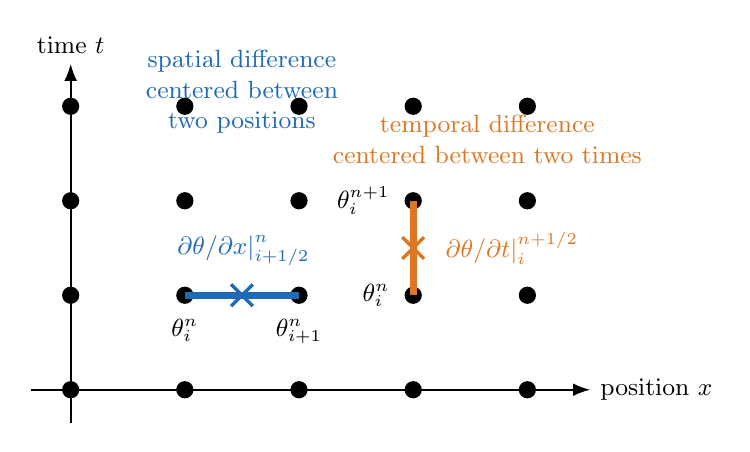
\begin{tikzpicture}[
    x=1.45cm,
    y=1.20cm,
    >=Latex,
    node/.style={circle,fill=black,inner sep=2.2pt},
    midpoint/.style={cross out,draw,line width=1.2pt,minimum size=6pt},
    every node/.style={font=\small}
]
  \draw[->,line width=0.7pt] (-0.35,0) -- (4.55,0) node[right] {position $x$};
  \draw[->,line width=0.7pt] (0,-0.35) -- (0,3.45) node[above] {time $t$};

  \foreach \i in {0,...,4}
    \foreach \n in {0,...,3}
      \node[node] at (\i,\n) {};

  \draw[spaceblue,line width=2.6pt] (1,1) -- (2,1);
  \node[midpoint,spaceblue] at (1.5,1) {};
  \node[spaceblue,above=7pt] at (1.5,1) {$\left.\partial\theta/\partial x\right|_{i+1/2}^{n}$};
  \node[below=5pt] at (1,1) {$\theta_i^n$};
  \node[below=5pt] at (2,1) {$\theta_{i+1}^n$};

  \draw[timeorange,line width=2.6pt] (3,1) -- (3,2);
  \node[midpoint,timeorange] at (3,1.5) {};
  \node[timeorange,right=7pt,align=left] at (3,1.5)
    {$\left.\partial\theta/\partial t\right|_{i}^{n+1/2}$};
  \node[left=5pt] at (3,1) {$\theta_i^n$};
  \node[left=5pt] at (3,2) {$\theta_i^{n+1}$};

  \node[align=center,text width=4.4cm,spaceblue] at (1.5,3.15)
    {spatial difference\\centered between two positions};
  \node[align=center,text width=4.4cm,timeorange] at (3.65,2.65)
    {temporal difference\\centered between two times};
\end{tikzpicture}
\end{document}
